\section{Methods for Markov chains}
\label{m:sec:methods}

\subsection{Discrete-time methods}
\label{m:sec:dt-methods}

\subsubsection{First-step analysis}
\label{m:sec:firststep}

A recurring discrete-time device, used for hitting probabilities and for the
Galton--Watson extinction probability in \cref{m:sec:gw}, is \emph{first-step}
(or one-step) analysis. Let $(X_n)_{n\ge0}$ be a discrete-time Markov chain on a
countable state space $\mathcal S$, and let $A\subset\mathcal S$ be a target set.
Write $h_i = \pr{X\text{ hits }A\mid X_0=i}$. Conditioning on the first transition
and using the Markov property yields the linear system
\begin{equation}
\label{m:eq:firststep}
h_i = 1\quad(i\in A),
\qquad
h_i = \sum_{j\in\mathcal S} P_{ij}\,h_j\quad(i\notin A),
\end{equation}
where $P$ is the one-step transition matrix. The same idea produces mean hitting
times, with an inhomogeneous term $+1$ on the right-hand side for transient states.
In continuous time the analogous identities come from the generator rather than from
$P$; both versions appear repeatedly below.

\subsubsection*{Generating functions and functional iteration}

For Galton--Watson processes the offspring \pgf{} $\phi$ iterates to give the law of
$Z_n$. Survival probabilities satisfy a closed nonlinear recursion such as
\cref{m:eq:SnIter}. Functional iteration, first-step analysis, and---later---product
and series manipulations of the survival amplitude $A(p)$ are the discrete-time
methods used in this thesis. The amplitude theory, including the identification of
$A(p)$ with a value of the Koenigs linearising function of the logistic map, is
developed in full in \ChA. The present chapter uses only the definition of $A(p)$ and
the conditional-mean formula of \cref{m:sec:condmeans}.

\subsection{Continuous-time methods}
\label{m:sec:ct-methods}

Throughout this subsection the linear birth--death process of \cref{m:sec:linbd} is
the running example. The same pattern---generator to master equation to
generating-function PDE to moments---applies to birth--death--catastrophe and
absorption models.

\subsubsection*{Backward equations and the generator}

For a continuous-time Markov chain with generator $Q$, the transition semigroup
$P(t)$ satisfies the Kolmogorov backward and forward equations
$\dot P = QP = PQ$. Applied to a bounded observable $f$, the function
$u_i(t)=\ex{f(X_t)\mid X_0=i}$ solves $\dot u = Qu$ with $u(0)=f$. First-step
reasoning in continuous time is the expansion of this equation over an infinitesimal
holding time.

\subsubsection*{Mean population size}

For linear birth--death rates $q_{n,n+1}=\lambda n$, $q_{n,n-1}=\mu n$, the mean
$m(t)=\ex{X_t}$ closes:
\begin{equation}
\label{m:eq:bdmean-method}
\dot m = (\lambda-\mu)m,
\qquad m(t)=m(0)\,\ee^{(\lambda-\mu)t},
\end{equation}
as in \cref{m:eq:bdmean}. Higher moments satisfy linear ODEs obtained by
differentiating the generating-function PDE of \cref{m:eq:bdpde}.

\subsubsection*{Variance and higher moments}

Differentiating the probability generating function (or the moment generating
function) along the PDE yields a hierarchy of moment equations. For linear
birth--death processes the continuous-time second-moment ODEs follow from
\cref{m:eq:bdpde} by the same route used for the mean. Explicit formulae are
omitted here when they are not needed for later chapters.

\subsubsection*{Hitting probabilities}

Let $A\subset\mathcal S$ be a target set for a continuous-time chain. The hitting
probabilities $h_i=\pr{\text{hit }A\mid X_0=i}$ solve the linear system
\begin{equation}
\label{m:eq:hitting}
\sum_j q_{ij}h_j = 0\quad(i\notin A),
\qquad h_i=1\quad(i\in A),
\end{equation}
with the boundary condition $h=0$ on any other absorbing class if required. For
birth--death processes on an interval the system reduces to a second-order difference
equation, solvable by summation exactly as in the discrete-time gambler's-ruin
calculation.

\subsubsection*{Extinction probabilities}

For continuous-time birth--death processes started at $n$, the ultimate extinction
probability $\eta_n$ solves a first-step balance using $\lambda$ and $\mu$; for the
linear case, $\eta_1=\min(1,\mu/\lambda)$. In discrete time the extinction probability
of a Galton--Watson process is the smallest non-negative root of $s=\phi(s)$. Both
facts are classical \cite{Athreya1972,Kendall1948}.

\subsubsection*{Conditional means}
\label{m:sec:condmeans}

For the subcritical binary Galton--Watson process ($p<\tfrac12$), late-time survival
obeys
\begin{equation}
\label{m:eq:lateS}
S_n \sim A(p)\,(2p)^n,
\qquad
A(p)=\lim_{n\to\infty}\frac{S_n}{(2p)^n},
\end{equation}
and the conditional mean converges to the reciprocal of this constant:
\begin{equation}
\label{m:eq:qsmean}
\ex{Z_n\mid Z_n>0}\;\xrightarrow{n\to\infty}\;\frac{1}{A(p)}.
\end{equation}
Existence of the Yaglom (quasi-stationary) limit is classical
\cite{Yaglom1947,Meleard2012,Collet2013}. The structure of $A(p)$ itself---product and
series representations, bounds, near-critical asymptotics, and the obstruction to an
elementary closed form---is the subject of \ChA.

\paragraph{Continuous-time closed form.}
\label{m:sec:cts}

The continuous-time linear birth--death process admits a closed form for its
Kolmogorov constant, developed here in basic detail. By contrast, the discrete
constant $A(p)$ has no known elementary formula; its full analytic theory is deferred
to \ChA.

Take the linear birth--death process of \cref{m:sec:linbd}, with per-capita birth
rate $\lambda$ and death rate $\mu$, started from $N$ individuals. Its extinction
probability $p_0(t)$ is \cref{m:eq:p0t}, and its survival probability is
$S^{(N)}(t) = 1-p_0(t)$.

\subsubsection*{Limiting mean conditioned on non-extinction}

The process has a stationary conditional mean when $\mu>\lambda$, that is in the
subcritical case. Exactly as in \cref{m:sec:condmeans},
\begin{equation}
\label{m:eq:condit}
\ex{X_t\mid X_t>0} = \frac{\ex{X_t}}{S^{(N)}(t)},
\end{equation}
and the late-time limit follows on applying L'Hôpital's rule. It is quicker to take
$N=1$ and compute directly. With $\ex{X_t}=\ee^{(\lambda-\mu)t}$ from
\cref{m:eq:bdmean} and
\begin{equation*}
S(t) = 1-\frac{\mu-\mu\ee^{(\mu-\lambda)t}}{\lambda-\mu\ee^{(\mu-\lambda)t}}
= \frac{\lambda-\mu}{\lambda-\mu\ee^{(\mu-\lambda)t}},
\end{equation*}
\cref{m:eq:condit} gives
\begin{equation*}
\ex{X_t\mid X_t>0} = \frac{\lambda\ee^{(\lambda-\mu)t}-\mu}{\lambda-\mu} .
\end{equation*}
For $\mu>\lambda$ the exponential decays, and the limiting conditional mean is the
constant
\begin{equation}
\label{m:eq:ctsqsmean}
\lim_{t\to\infty}\ex{X_t\mid X_t>0} = \frac{\mu}{\mu-\lambda}
= \frac{1}{1-\lambda/\mu}
\;\lrb{=\frac{1}{\Ac}} .
\end{equation}
\Cref{m:fig:bd-condmean} shows the approach of the conditional mean to this limit for
a representative subcritical pair $(\lambda,\mu)$. To compare this with the
discrete-time constant the two parametrisations must be matched, and
\cref{m:prop:race} is what matches them: with birth and death clocks running at rates
$\lambda$ and $\mu$, the probability that the birth clock wins is
$p = \lambda/(\lambda+\mu)$, so that $\lambda/\mu = p/(1-p)$. In that
parametrisation
\begin{equation}
\label{m:eq:Acts}
\frac{1}{\Ac} = \frac{1-p}{1-2p},
\qquad\text{that is}\qquad
\Ac(p) = \frac{1-2p}{1-p} ,
\end{equation}
the subscript marking this as the continuous-time constant, to distinguish it from
the discrete-time $A(p)$ of \cref{m:eq:lateS}.

\begin{figure}[ht]
\centering
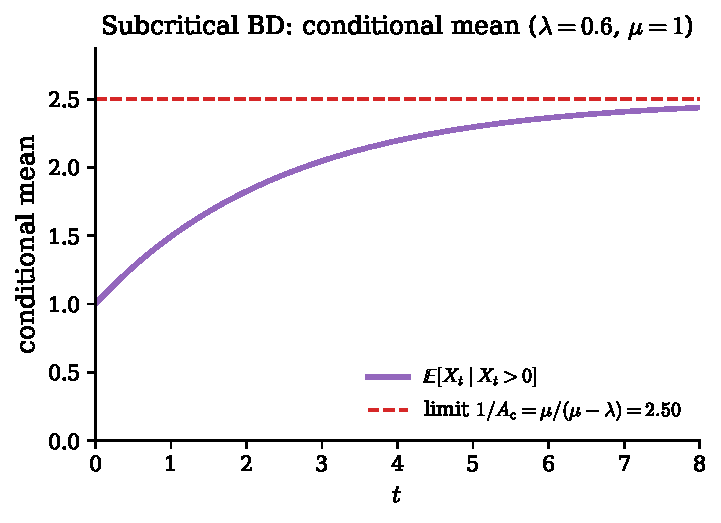
\includegraphics[width=0.58\textwidth]{figures/tikz_gen/bd_conditional_mean.pdf}
\caption{Subcritical linear birth--death process: the conditional mean
$\ex{X_t\mid X_t>0}$ rises from $1$ to the stationary value
$1/\Ac=\mu/(\mu-\lambda)$ (dashed). Parameters $\lambda=0.6$, $\mu=1$.}
\label{m:fig:bd-condmean}
\end{figure}

\begin{figure}[ht]
\centering
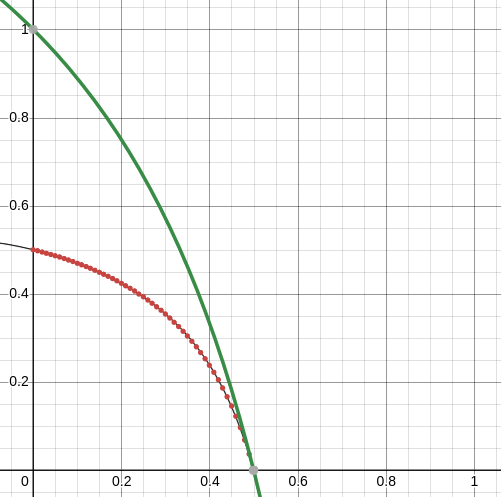
\includegraphics[width=0.5\textwidth]{figures/IMG_ch3/dtctA.png}
\caption{The continuous-time constant $\Ac(p)=(1-2p)/(1-p)$ (green) against
high-precision numerical values of the discrete-time constant $A(p)$ (red points).
Both vanish at $p=\tfrac12$; at $p=0$ the continuous curve starts at $1$ and the
discrete one at $\tfrac12$, and the two are not related by a constant factor in
between. The black line is a symbolic-regression candidate discussed in \ChA; it tracks
the points closely but is not exact. The exact relation between $A$ and $\Ac$ is
established in \ChA.}
\label{m:fig:dtct}
\end{figure}

\Cref{m:fig:dtct} plots $\Ac(p)$ against numerically obtained values of $A(p)$ and
raises a natural question: why does the continuous curve start at $1$ and the discrete
one at $\tfrac12$? Merely halving $\Ac$ does not superpose them, because at the other
end of the range they meet. As shown in \ChA, $\Ac(p)/2$ is an exact lower bound for
$A(p)$, attained only as $p\to0$, while near criticality both constants share the
leading asymptotic $2(1-2p)$. The product, series, bounds, and dynamical obstruction
for discrete $A(p)$ occupy \ChA.

The continuous-time constant is elementary because the generating-function PDE closes.
The discrete constant $A(p)$ is not known to admit an elementary formula; that contrast,
and the full discrete theory, occupy \ChA.

\subsection{Method of characteristics}
\label{m:sec:moc}

Generating-function equations for continuous-time population models are first-order
linear PDEs. The method of characteristics converts such a PDE into a system of
ordinary differential equations along curves in the $(t,x)$ (or multi-variable) space
(\cref{m:fig:moc-schematic}). The presentation below is organised for readability: the
method is checked on the absorption--death model, whose answer is already known by an
independence argument, and the longer absorption--birth--death closed form is recorded
in \cref{m:app:moc-extended}.

\begin{figure}[ht]
\centering
\begin{tikzpicture}[
  font=\small,
  >=Latex,
  declare function={
    charA(\t)=0.35+0.55*\t+0.04*\t*\t;
    charB(\t)=1.4+0.35*\t;
    charC(\t)=2.55+0.22*\t-0.01*\t*\t;
  }
]
  % Axes
  \draw[->, thick] (-0.15,0) -- (5.6,0) node[right] {$t$};
  \draw[->, thick] (0,-0.15) -- (0,3.5) node[above] {$x$};

  % Initial surface t=0
  \draw[thick, Mgray, densely dashed] (0,0.2) -- (0,3.2);
  \node[font=\scriptsize, text=Mgray, rotate=90, anchor=south] at (-0.35,1.7)
    {initial surface $t=0$};

  % Characteristic curves
  \draw[thick, Mblue, domain=0:4.6, samples=60, smooth]
    plot ({\x},{charA(\x)});
  \draw[thick, Mgreen!60!black, domain=0:4.6, samples=60, smooth]
    plot ({\x},{charB(\x)});
  \draw[thick, Morange, domain=0:4.6, samples=60, smooth]
    plot ({\x},{charC(\x)});

  % Markers on initial surface
  \fill[Mblue] (0,{charA(0)}) circle (1.6pt);
  \fill[Mgreen!60!black] (0,{charB(0)}) circle (1.6pt);
  \fill[Morange] (0,{charC(0)}) circle (1.6pt);

  % Point evaluation
  \coordinate (P) at (3.2,{charB(3.2)});
  \fill[Mred] (P) circle (2.0pt);
  \node[font=\scriptsize, above right=-1pt] at (P) {$(t,x)$};
  \draw[Mred, densely dotted] (P) -- (0,{charB(0)});
  \node[font=\scriptsize, text=Mred!70!black, left] at (-0.05,{charB(0)})
    {$\sigma$};

  % Annotation
  \node[align=left, font=\scriptsize, text=Mgray] at (7.35,2.4)
    {Along each curve:\\[2pt]
     PDE $\;\to\;$ ODEs\\[1pt]
     $G$ constant (or\\[1pt]
     simple transport)};
  \draw[->, Mgray] (5.9,1.7) to[out=180,in=0] (4.3,{charB(4.0)});

  \node[font=\scriptsize, text=Mblue] at (4.9,0.55) {characteristics};
\end{tikzpicture}
\caption{Schematic of the method of characteristics for a first-order linear PDE in
$(t,x)$. Solution values at a point $(t,x)$ are recovered by integrating the
characteristic ODEs back to the initial surface $t=0$, where $G$ is known. In the
absorption models the same idea is applied in $(t,x,y)$ with a two-dimensional
initial surface.}
\label{m:fig:moc-schematic}
\end{figure}

\subsubsection{Worked example: absorption--death}
\label{m:sec:absdeath}

A particle resident in a compartment may die. Keeping $X_t$ and $Y_t$ for the
interior and exterior counts, the two channels are absorption from the exterior
medium into the compartment at per-particle rate $\alpha$, and death inside at
per-particle rate $\mu$ (\cref{m:fig:abs-compartment}). The infinitesimal rates
read
\begin{align*}
\pr{\Delta X = 1,\ \Delta Y = -1 \mid Y_t=j} &= j\alpha\,\Delta t, &&\text{(absorption)}\\
\pr{\Delta X = -1,\ \Delta Y = 0 \mid X_t=i} &= i\mu\,\Delta t, &&\text{(death)}\\
\pr{\Delta X = 0,\ \Delta Y = 0 \mid X_t=i,\ Y_t=j} &= 1-(j\alpha+i\mu)\Delta t, &&\text{(no event)}
\end{align*}

\begin{figure}[ht]
\centering
\begin{tikzpicture}[
  font=\small,
  >=Latex,
  box/.style={
    draw, thick, rounded corners=4pt,
    minimum width=3.4cm, minimum height=2.5cm,
    align=center
  }
]
  % Exterior medium Y
  \node[box, draw=Mblue!75!black, fill=Mblue!8] (Y) at (0,0) {};
  \node[font=\bfseries, text=Mblue!70!black] at (0,0.85) {Exterior $Y$};
  \node[font=\normalsize] at (0,0.15) {$Y_t$ particles};
  \node[font=\scriptsize, text=Mgray] at (0,-0.55) {initial: $Y_0=N$};
  \node[font=\scriptsize, text=Mgray] at (0,-1.0) {no internal dynamics};

  % Interior compartment X
  \node[box, draw=Mgreen!55!black, fill=Mgreen!8] (X) at (6.2,0) {};
  \node[font=\bfseries, text=Mgreen!45!black] at (6.2,0.85) {Compartment $X$};
  \node[font=\normalsize] at (6.2,0.15) {$X_t$ particles};
  \node[font=\scriptsize, text=Mgray] at (6.2,-0.55) {initial: $X_0=0$};
  \node[font=\scriptsize, text=Mgray] at (6.2,-1.0) {death only};

  % Absorption arrow Y -> X
  \draw[->, very thick, Mblue]
    (Y.east) -- node[above, font=\small, text=Mblue!70!black] {$j\alpha$}
    node[below, font=\scriptsize, text=Mgray] {absorption} (X.west);

  % Death arrow leaving X
  \draw[->, very thick, Mred!75!black]
    (X.south) -- ++(0,-1.15)
    node[midway, right, font=\small, text=Mred!70!black] {$i\mu$}
    node[midway, left, font=\scriptsize, text=Mgray] {death};
  \node[font=\scriptsize, text=Mred!65!black] at (6.2,-1.55) {removed};

  % Particle counts annotation
  \node[draw=Mpurple!60, fill=Mpurple!6, rounded corners=3pt, thick,
        align=left, font=\scriptsize, inner sep=5pt]
    at (3.1,2.05) {
      rates when $(X_t,Y_t)=(i,j)$:\\[2pt]
      absorption: $j\alpha$ \quad
      death: $i\mu$
    };

  % Small particle icons (schematic dots)
  \foreach \k in {0,...,4} {
    \fill[Mblue!80] (-0.9+0.35*\k, -0.05) circle (2.2pt);
  }
  \node[font=\tiny, text=Mblue!70!black] at (0.95,-0.05) {$\cdots$};

  \foreach \k in {0,...,2} {
    \fill[Mgreen!70!black] (5.55+0.35*\k, -0.05) circle (2.2pt);
  }
\end{tikzpicture}
\caption{Absorption--death compartment schematic. Particles start in the exterior
medium $Y$ (count $Y_t$, initially $N$). Each exterior particle is absorbed into the
compartment $X$ at rate $\alpha$, contributing the total absorption rate $j\alpha$
when $Y_t=j$. Inside $X$, each of the $i$ residents dies independently at rate
$\mu$, for total death rate $i\mu$. There is no birth in this model.}
\label{m:fig:abs-compartment}
\end{figure}

with forward Kolmogorov equations
\begin{equation}
\label{m:eq:FK2}
\ddt{p_{i,j}} = \alpha(j+1)p_{i-1,j+1} + \mu(i+1)p_{i+1,j} - (\alpha j+\mu i)p_{i,j} .
\end{equation}
The derivation of \cref{m:sec:absonly} carries over unchanged and gives the
first-order linear equation
\begin{equation}
\label{m:eq:PDE2}
\pddt{G} = \mu(1-x)\pdd{G}{x} + \alpha(x-y)\pdd{G}{y},
\qquad G(x,y,0) = y^N ,
\end{equation}
and the same difficulty. Once again the solution can be constructed via
\cref{m:eq:indRelPGF}, since individual particles remain independent.

Without birth events the number of particles cannot exceed its initial value, so
for an isolated particle the generating function has just three terms,
\begin{equation*}
G_1(x,y,t) = p_{0,0}(t) + p_{1,0}(t)\,x + p_{0,1}(t)\,y .
\end{equation*}
The state probabilities follow from
\begin{equation*}
\ddt{p_{0,1}} = -\alpha p_{0,1},
\qquad
\ddt{p_{1,0}} = \alpha p_{0,1} - \mu p_{1,0},
\end{equation*}
whence
\begin{equation}
\label{m:eq:absdeathstates}
p_{0,1}(t) = \ee^{-\alpha t},
\qquad
p_{1,0}(t) = \frac{\alpha}{\mu-\alpha}\lrb{\ee^{-\alpha t}-\ee^{-\mu t}},
\qquad
p_{0,0}(t) = 1-p_{0,1}(t)-p_{1,0}(t),
\end{equation}
plotted in \cref{m:fig:abs2}. Applying \cref{m:eq:indRelPGF} gives the general
generating function
\begin{equation}
\label{m:eq:Gabsdeath}
G_n(x,y,t) = \Bigl(
1-\tfrac{\mu}{\mu-\alpha}\ee^{-\alpha t} + \tfrac{\alpha}{\mu-\alpha}\ee^{-\mu t}
+ \tfrac{\alpha}{\mu-\alpha}\bigl(\ee^{-\alpha t}-\ee^{-\mu t}\bigr)x
+ \ee^{-\alpha t}y\Bigr)^n .
\end{equation}

\begin{figure}[H]
\centering
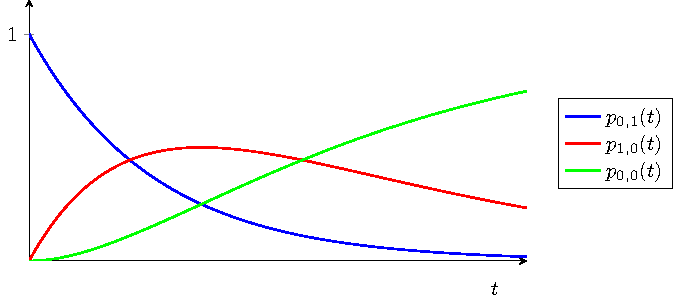
\includegraphics[width=0.62\textwidth]{figures/IMG_ch3/abs2.pdf}
\caption{State probabilities for the single-particle absorption--death model,
\cref{m:eq:absdeathstates}. The particle starts outside ($p_{0,1}$, blue), is
absorbed into the compartment ($p_{1,0}$, red, which rises and then decays as death
takes over), and finally dies ($p_{0,0}$, green, absorbing).}
\label{m:fig:abs2}
\end{figure}


\subsubsection{Characteristics applied to absorption--death}
\label{m:sec:mocabsdeath}

Before continuing to absorption--birth--death, where replication may occur inside
the compartment and the independence shortcut is unavailable, it is worth
revisiting absorption--death from the point of view of its partial differential
equation. Having \cref{m:eq:Gabsdeath} already in hand makes it an ideal test
case.\footnote{I am grateful to Benjamin Sharp for the advice on applying the
method of characteristics to three-variate problems that unlocked this section.}

Introduce a change of variables $(x,y,t)\to(\sigma,\eta,\tau)$, writing
\begin{equation*}
G(x,y,t) = G\bigl(x(\sigma,\eta,\tau),\,y(\sigma,\eta,\tau),\,t(\sigma,\eta,\tau)\bigr)
\equiv G(\sigma,\eta,\tau).
\end{equation*}
The method seeks solutions along the characteristic curves of constant $\sigma$ and
$\eta$, on which $G$ is a function of $\tau$ alone. To fix the parametrisation we
impose an initial surface,
\begin{equation}
\label{m:eq:ICpar}
x(\sigma,\eta,0) = \sigma,
\qquad
y(\sigma,\eta,0) = \eta,
\qquad
t(\sigma,\eta,0) = 0 .
\end{equation}
With $G$ a function of $\tau$ only along a characteristic, the chain rule gives
\begin{equation*}
\dda{G}{\tau} = \pddt{G}\dda{t}{\tau} + \pdd{G}{x}\dda{x}{\tau} + \pdd{G}{y}\dda{y}{\tau},
\end{equation*}
which is to be compared with \cref{m:eq:PDE2} written as
\begin{equation*}
0 = -\pddt{G} + \mu(1-x)\pdd{G}{x} + \alpha(x-y)\pdd{G}{y} .
\end{equation*}
Comparing coefficients yields the characteristic system
\begin{align}
\dda{G}{\tau} &= 0, \label{m:eq:ch11}\\
\dda{t}{\tau} &= -1, \label{m:eq:ch12}\\
\dda{x}{\tau} &= \mu(1-x), \label{m:eq:ch13}\\
\dda{y}{\tau} &= \alpha(x-y). \label{m:eq:ch14}
\end{align}

\paragraph{The equation for $G$, \eqref{m:eq:ch11}.}
$G$ is constant along characteristics, so $G$ is a function of $(\sigma,\eta)$
alone. Under \cref{m:eq:ICpar} the initial condition $G(x,y,0)=y^N$ becomes
$G(\sigma,\eta,0)=\eta^N$, so
\begin{equation}
\label{m:eq:GetaN}
G(\sigma,\eta,\tau) = \eta^N .
\end{equation}
The whole problem thus reduces to expressing $\eta$ in terms of $(x,y,t)$.

\paragraph{The equation for $t$, \eqref{m:eq:ch12}.}
Integrating gives $t = -\tau + c(\sigma,\eta)$, and \cref{m:eq:ICpar} fixes $c=0$:
\begin{equation}
\label{m:eq:minustau}
t = -\tau .
\end{equation}
The characteristic parameter runs backwards in time, which is what allows the
initial surface to be reached from any $(x,y,t)$.

\paragraph{The equation for $x$, \eqref{m:eq:ch13}.}
Separating variables gives $1-x = c(\sigma,\eta)\ee^{-\mu\tau}$, and
\cref{m:eq:ICpar} gives $c = 1-\sigma$:
\begin{equation}
\label{m:eq:sandxwithtau}
1-x = (1-\sigma)\ee^{-\mu\tau} .
\end{equation}

\paragraph{The equation for $y$, \eqref{m:eq:ch14}.}
Substituting \cref{m:eq:sandxwithtau},
\begin{equation*}
\dda{y}{\tau} = \alpha\bigl(1-(1-\sigma)\ee^{-\mu\tau}-y\bigr),
\end{equation*}
and solving with integrating factor $\ee^{\alpha\tau}$,
\begin{equation*}
y = 1-\frac{\alpha}{\alpha-\mu}(1-\sigma)\ee^{-\mu\tau} + c(\sigma,\eta)\ee^{-\alpha\tau} .
\end{equation*}
Applying \cref{m:eq:ICpar} gives
$c(\sigma,\eta) = \eta + \frac{\alpha}{\alpha-\mu}(1-\sigma)-1$, so
\begin{equation}
\label{m:eq:ywitheta}
y = 1-\frac{\alpha}{\alpha-\mu}(1-\sigma)\ee^{-\mu\tau}
+ \lrb{\eta + \frac{\alpha}{\alpha-\mu}(1-\sigma)-1}\ee^{-\alpha\tau} .
\end{equation}

\paragraph{Recovering the solution.}
Rearranging \cref{m:eq:ywitheta} for $\eta$, substituting $\sigma$ from
\cref{m:eq:sandxwithtau} and $\tau=-t$ from \cref{m:eq:minustau}, gives
\begin{equation*}
\eta = 1-\frac{\mu}{\mu-\alpha}\ee^{-\alpha t} + \frac{\alpha}{\mu-\alpha}\ee^{-\mu t}
+ \frac{\alpha}{\mu-\alpha}\bigl(\ee^{-\alpha t}-\ee^{-\mu t}\bigr)x
+ \ee^{-\alpha t}y ,
\end{equation*}
and \cref{m:eq:GetaN} then reproduces \cref{m:eq:Gabsdeath} exactly. The two routes
agree, and the machinery is ready for the case in which only one of them is
available.



\begin{remark}[Further absorption models]
\label{m:rem:moc-app}
Absorption-only and absorption--birth--death generating functions, including the
hypergeometric closed form and resonance discussion, are collected in
\cref{m:app:moc-extended}. The hypergeometric integral identity and coefficient
extraction lemmas remain in \cref{m:app:hyp,m:app:extract}.
\end{remark}
